\section{The workload is a sequence of interrupted computations}\label{sec:C31:01}
Agentic serving is a workload of correlated model calls separated by tools, waiting, branching, and state updates. The prompt of the next call often overlaps a prior prompt, but its useful overlap depends on serialization, context editing, and model compatibility. A tool can pause generation long enough for a cache to be evicted; several workers can share an initial prefix and then diverge; a resumed session can return to another serving replica. A benchmark that repeatedly decodes independent fixed-length prompts misses these interactions.

Represent a session by turns $j=1,\ldots,J$, each with input length $I_j$, generated length $O_j$, reused prefix length $R_j$, tool duration $Z_j$, and state-transform identifier $v_j$. For serial calls whose tool waits do not overlap model work, elapsed time is
\begin{equation}
 T_{\rm session}=\sum_j
 \left[W_j+T_{\rm prefill}(I_j,R_j,v_j)
 +T_{\rm decode}(O_j,I_j)+Z_j\right],
\end{equation}
where $W_j$ includes admission and scheduling delay. This equality is an accounting identity for that serial workload. Speculative tool execution, parallel workers, and overlapping serving stages require a dependency graph whose critical path replaces the sum; adding overlapping durations would double-count time. Reporting model time alone omits delays that often determine whether an agent finishes within its deadline.

The September 2026 vLLM AgentX engineering account explicitly treats multi-turn agent traffic, prefix reuse, scheduling, and prefill/decode disaggregation as a coupled serving problem. Its reported throughput and cost comparisons are configuration- and workload-dependent vendor evidence. They cannot be transferred to arbitrary task completion or substituted for quality-matched end-to-end measurements~\cite{root_vllm2026agentx}. The analysis below therefore derives resource constraints under explicit hypothetical assumptions and identifies what a measurement must establish.

The serving policy itself can affect reasoning and memory behavior. Aggressive truncation changes observations. A timeout can cause the harness to retry and consume a different random continuation. Admission control can alter which parallel branch finishes first and therefore which evidence a selector sees. These are changes in the executed policy, even when the model weights are fixed. Performance optimization should preserve the declared behavioral contract or measure the consequences of changing it.


% SCIENTIFIC_FIGURE_C31
Figure~\ref{fig:C31:overview} distinguishes cache placement from the computational identity required for reuse.
\begin{figure}[!htbp]
\centering
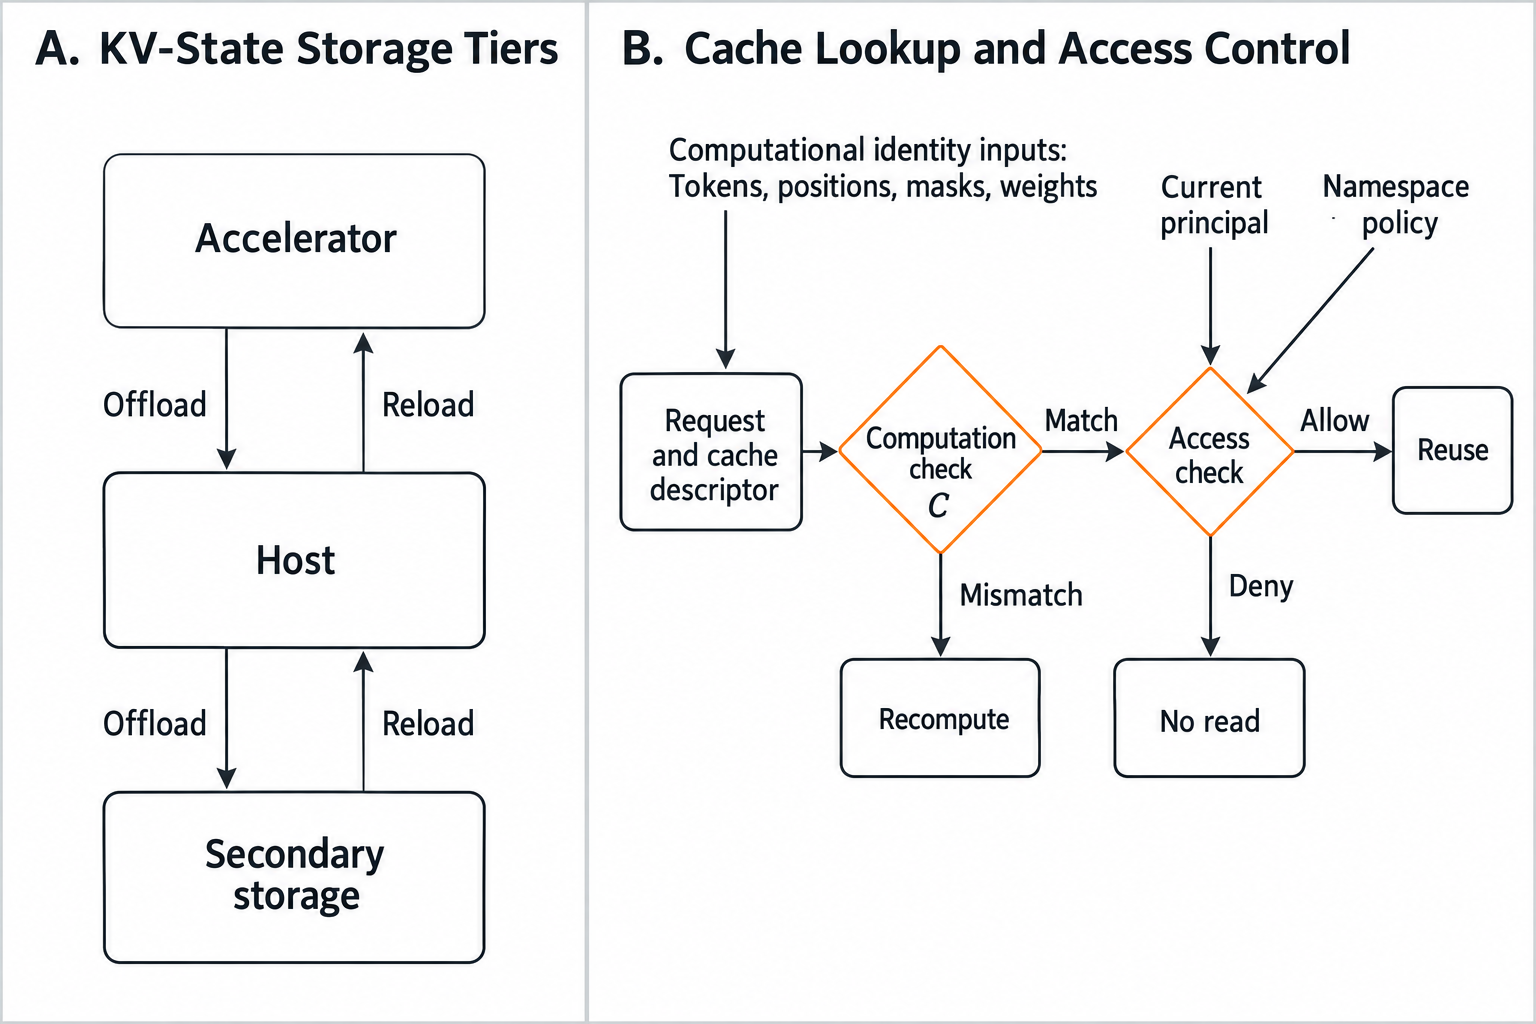
\includegraphics[width=\linewidth]{book/figures/assets/F31review.png}
\caption{Tier placement, computational compatibility and permission to read are separate cache questions. The figure-local $C$ is a computational-match predicate. The listed identity inputs are illustrative; a valid key covers every dependency in the declared forward pass. Descriptor lookup is namespace-scoped, and reuse requires current access authorization. A storage hit does not establish a latency benefit; mismatches need valid recomputation.}
\label{fig:C31:overview}
\end{figure}
